\chapter{XSL}

\section{Conception}

Dans un premier temps, nous avions choisi de suivre une conception orientée objet, et c'est donc
naturellement que nous avons proposé une classe dédiée aux documents \textit{XSL}, proposant les
fonctionnalités de transformation d'une feuille XSL, et de même pour les instructions \textit{XSL}.

\begin{figure}[h!]
    \centering
    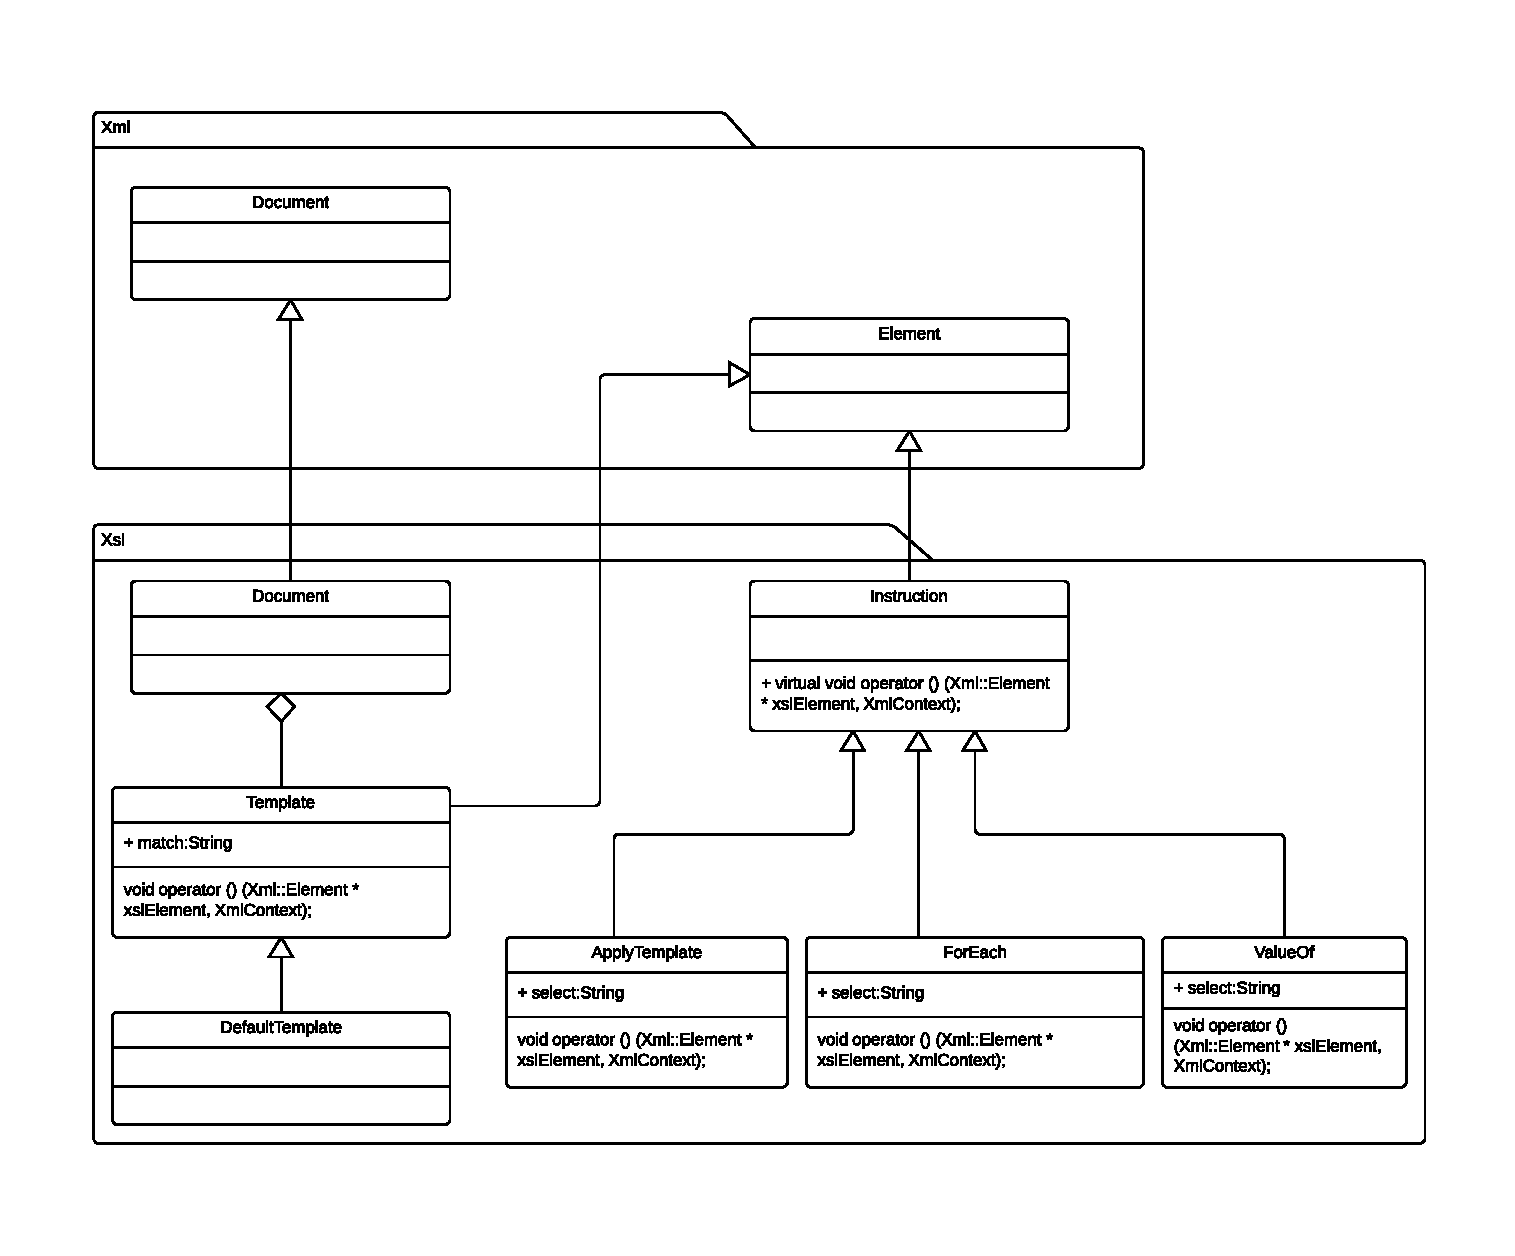
\includegraphics[width=\linewidth]{images/xsl-uml-old.pdf}
    \caption{Ancienne conception du module XSL}
    \label{oldXslClassDiagram}
\end{figure}

Néanmoins, cette conception présente de nombreux inconvénients :

\begin{enumerate}
    \item Cast des éléments XML.
    \item Cast des éléments XML.
    \item Cast des éléments XML.
    \item Cast des éléments XML.
\end{enumerate}

\begin{landscape}
\begin{figure}[h!]
    \centering
    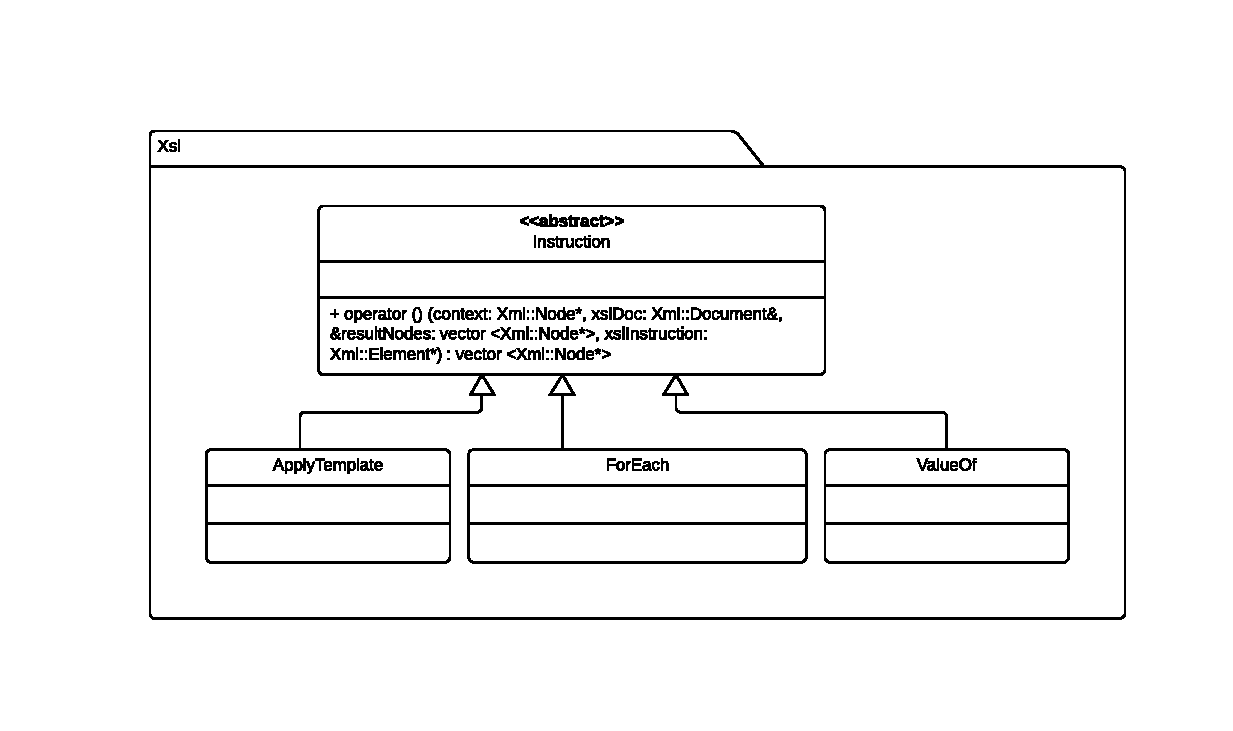
\includegraphics[width=\linewidth]{images/xsl-uml.pdf}
    \caption{Diagramme de classe des instructions XSL}
    \label{xslClassDiagram}
\end{figure}
\end{landscape}


\section{Algorithme}

